\section{Technical Regulations}


\subsection{Positioning}
The challenge will take place in a hangar at the Manching Airport (48°43'21.7"N 11°33'04.9"E).
To imporve the state estimation in a potential gps denied environment, a camera based positioning system using ArUco marker can be used.
Two ArUco marker are attached to each pillar in the hangar.
The figure below illustrates the IDs of the maker that are attached to the pillars, where the lower ArUco marker is mounted at a height of 2m and the upper marker at 4m.

\begin{figure}[H]

\centering

\tikzset{every picture/.style={line width=0.75pt}} %set default line width to 0.75pt        

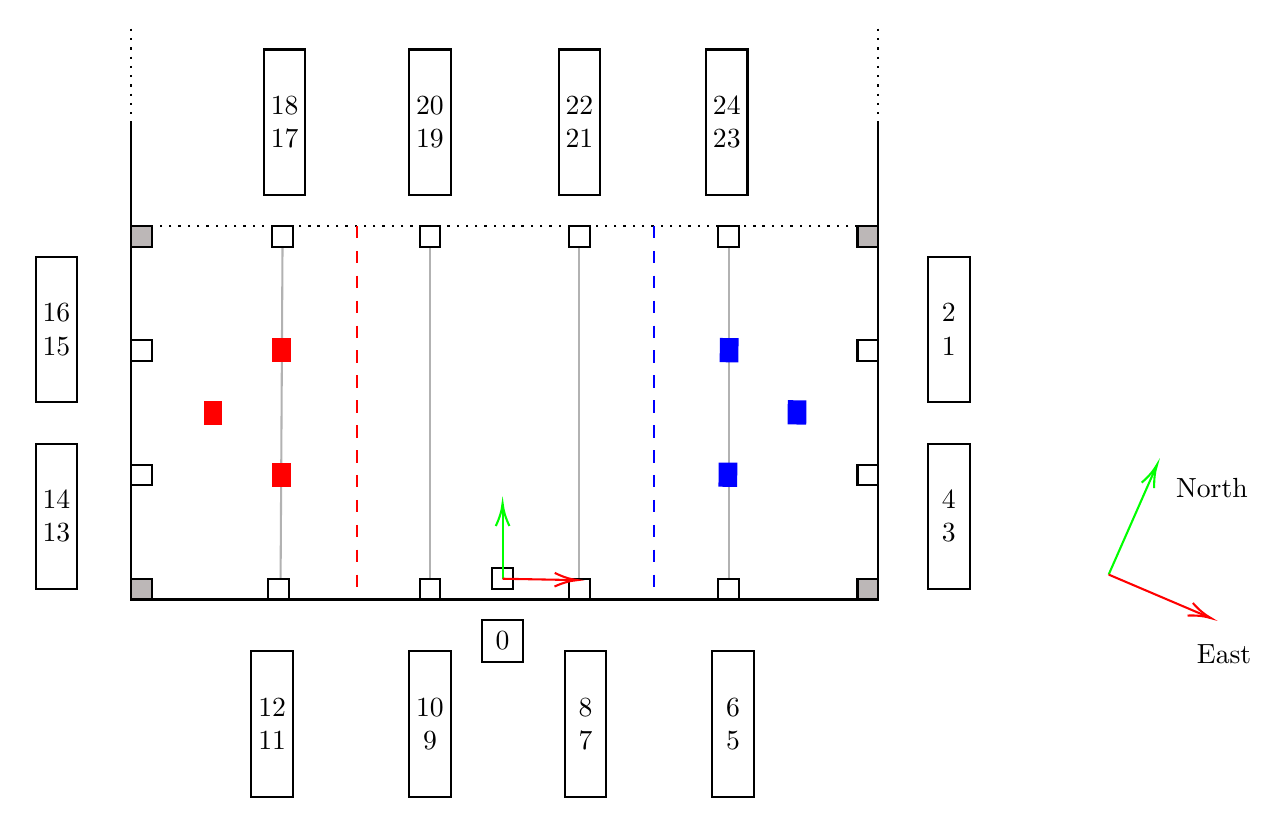
\begin{tikzpicture}[x=0.75pt,y=0.75pt,yscale=-1,xscale=1]
%uncomment if require: \path (0,403); %set diagram left start at 0, and has height of 403

%Straight Lines [id:da8324081494103803] 
\draw [color={rgb, 255:red, 178; green, 178; blue, 178 }  ,draw opacity=1 ]   (344,97.7) -- (344,275) ;
%Straight Lines [id:da9583452157235313] 
\draw [color={rgb, 255:red, 178; green, 178; blue, 178 }  ,draw opacity=1 ]   (272,97.7) -- (272,275) ;
%Shape: Rectangle [id:dp3433626255284923] 
\draw  [fill={rgb, 255:red, 188; green, 183; blue, 183 }  ,fill opacity=1 ] (56,265) -- (66,265) -- (66,275) -- (56,275) -- cycle ;
%Shape: Rectangle [id:dp6616954858549284] 
\draw  [fill={rgb, 255:red, 188; green, 183; blue, 183 }  ,fill opacity=1 ] (56,95) -- (66,95) -- (66,105) -- (56,105) -- cycle ;
%Shape: Rectangle [id:dp2948289764970793] 
\draw   (56,150) -- (66,150) -- (66,160) -- (56,160) -- cycle ;
%Shape: Rectangle [id:dp6971973555173374] 
\draw   (56,210) -- (66,210) -- (66,220) -- (56,220) -- cycle ;
%Shape: Rectangle [id:dp9126690703683185] 
\draw  [fill={rgb, 255:red, 188; green, 183; blue, 183 }  ,fill opacity=1 ] (406,265) -- (416,265) -- (416,275) -- (406,275) -- cycle ;
%Shape: Rectangle [id:dp36362493354229275] 
\draw  [fill={rgb, 255:red, 188; green, 183; blue, 183 }  ,fill opacity=1 ] (406,95) -- (416,95) -- (416,105) -- (406,105) -- cycle ;
%Shape: Rectangle [id:dp7438280632958825] 
\draw   (406,150) -- (416,150) -- (416,160) -- (406,160) -- cycle ;
%Shape: Rectangle [id:dp8190129040006575] 
\draw   (406,210) -- (416,210) -- (416,220) -- (406,220) -- cycle ;
%Straight Lines [id:da6821139759238273] 
\draw [color={rgb, 255:red, 178; green, 178; blue, 178 }  ,draw opacity=1 ]   (129,99.1) -- (128,271.63) ;
%Shape: Rectangle [id:dp12978164760841726] 
\draw  [fill={rgb, 255:red, 255; green, 255; blue, 255 }  ,fill opacity=1 ] (122,265) -- (132,265) -- (132,275) -- (122,275) -- cycle ;
%Shape: Rectangle [id:dp7976816015193462] 
\draw  [fill={rgb, 255:red, 255; green, 255; blue, 255 }  ,fill opacity=1 ] (124,95) -- (134,95) -- (134,105) -- (124,105) -- cycle ;
%Shape: Rectangle [id:dp9966657246268984] 
\draw  [fill={rgb, 255:red, 255; green, 255; blue, 255 }  ,fill opacity=1 ] (339,265) -- (349,265) -- (349,275) -- (339,275) -- cycle ;
%Shape: Rectangle [id:dp5757119210618549] 
\draw  [draw opacity=0][fill={rgb, 255:red, 255; green, 0; blue, 0 }  ,fill opacity=1 ] (124,209) -- (133,209) -- (133,220.67) -- (124,220.67) -- cycle ;
%Straight Lines [id:da32211068188423364] 
\draw    (56,45) -- (56,265) ;
%Straight Lines [id:da4667069569376905] 
\draw    (406,275) -- (66,275) ;
%Straight Lines [id:da936931704558561] 
\draw    (416,265) -- (416,45) ;
%Straight Lines [id:da9729387023000151] 
\draw  [dash pattern={on 0.84pt off 2.51pt}]  (406,95) -- (66,95) ;
%Straight Lines [id:da5555743691262991] 
\draw [color={rgb, 255:red, 178; green, 178; blue, 178 }  ,draw opacity=1 ]   (200,94.33) -- (200,271.63) ;
%Shape: Rectangle [id:dp7316698787727904] 
\draw  [fill={rgb, 255:red, 255; green, 255; blue, 255 }  ,fill opacity=1 ] (195,265) -- (205,265) -- (205,275) -- (195,275) -- cycle ;
%Shape: Rectangle [id:dp5859859750919403] 
\draw  [fill={rgb, 255:red, 255; green, 255; blue, 255 }  ,fill opacity=1 ] (267,265) -- (277,265) -- (277,275) -- (267,275) -- cycle ;
%Shape: Rectangle [id:dp1572370552698623] 
\draw  [fill={rgb, 255:red, 255; green, 255; blue, 255 }  ,fill opacity=1 ] (195,95) -- (205,95) -- (205,105) -- (195,105) -- cycle ;
%Shape: Rectangle [id:dp9841641512210579] 
\draw  [draw opacity=0][fill={rgb, 255:red, 255; green, 0; blue, 0 }  ,fill opacity=1 ] (124,149) -- (133,149) -- (133,160.67) -- (124,160.67) -- cycle ;
%Shape: Rectangle [id:dp039623004192071765] 
\draw  [draw opacity=0][fill={rgb, 255:red, 255; green, 0; blue, 0 }  ,fill opacity=1 ] (91,179.33) -- (100,179.33) -- (100,191) -- (91,191) -- cycle ;
%Shape: Rectangle [id:dp5350102750244554] 
\draw  [draw opacity=0][fill={rgb, 255:red, 0; green, 0; blue, 255 }  ,fill opacity=1 ] (348.58,160.75) -- (339.58,160.67) -- (339.69,149) -- (348.69,149.09) -- cycle ;
%Shape: Rectangle [id:dp8150990393346593] 
\draw  [draw opacity=0][fill={rgb, 255:red, 0; green, 0; blue, 255 }  ,fill opacity=1 ] (348,220.75) -- (339,220.66) -- (339.11,209) -- (348.11,209.08) -- cycle ;
%Shape: Rectangle [id:dp37866285102082187] 
\draw  [draw opacity=0][fill={rgb, 255:red, 0; green, 0; blue, 255 }  ,fill opacity=1 ] (381.29,190.73) -- (372.29,190.65) -- (372.4,178.98) -- (381.4,179.07) -- cycle ;
%Shape: Rectangle [id:dp3600599674807883] 
\draw  [fill={rgb, 255:red, 255; green, 255; blue, 255 }  ,fill opacity=1 ] (339,95) -- (349,95) -- (349,105) -- (339,105) -- cycle ;
%Shape: Rectangle [id:dp4499187841739831] 
\draw  [fill={rgb, 255:red, 255; green, 255; blue, 255 }  ,fill opacity=1 ] (267,95) -- (277,95) -- (277,105) -- (267,105) -- cycle ;
%Straight Lines [id:da4108053166014911] 
\draw [color={rgb, 255:red, 0; green, 255; blue, 0 }  ,draw opacity=1 ]   (527,263) -- (549.53,211.83) ;
\draw [shift={(550.33,210)}, rotate = 113.76] [color={rgb, 255:red, 0; green, 255; blue, 0 }  ,draw opacity=1 ][line width=0.75]    (10.93,-3.29) .. controls (6.95,-1.4) and (3.31,-0.3) .. (0,0) .. controls (3.31,0.3) and (6.95,1.4) .. (10.93,3.29)   ;
%Straight Lines [id:da8518368663842253] 
\draw [color={rgb, 255:red, 255; green, 0; blue, 0 }  ,draw opacity=1 ]   (527,263) -- (574.49,283.22) ;
\draw [shift={(576.33,284)}, rotate = 203.06] [color={rgb, 255:red, 255; green, 0; blue, 0 }  ,draw opacity=1 ][line width=0.75]    (10.93,-3.29) .. controls (6.95,-1.4) and (3.31,-0.3) .. (0,0) .. controls (3.31,0.3) and (6.95,1.4) .. (10.93,3.29)   ;
%Shape: Rectangle [id:dp47541913233873645] 
\draw  [fill={rgb, 255:red, 255; green, 255; blue, 255 }  ,fill opacity=1 ] (230,260) -- (240,260) -- (240,270) -- (230,270) -- cycle ;
%Shape: Rectangle [id:dp7925913677020975] 
\draw   (440,110) -- (460,110) -- (460,180) -- (440,180) -- cycle ;
%Shape: Rectangle [id:dp5853821618437607] 
\draw   (440,200) -- (460,200) -- (460,270) -- (440,270) -- cycle ;
%Shape: Rectangle [id:dp8950595692026859] 
\draw   (336,300) -- (356,300) -- (356,370) -- (336,370) -- cycle ;
%Shape: Rectangle [id:dp8736581379567236] 
\draw   (265,300) -- (285,300) -- (285,370) -- (265,370) -- cycle ;
%Shape: Rectangle [id:dp7016375790720544] 
\draw   (190,300) -- (210,300) -- (210,370) -- (190,370) -- cycle ;
%Shape: Rectangle [id:dp6651707993087799] 
\draw   (114,300) -- (134,300) -- (134,370) -- (114,370) -- cycle ;
%Shape: Rectangle [id:dp28408371720304637] 
\draw   (10,200) -- (30,200) -- (30,270) -- (10,270) -- cycle ;
%Shape: Rectangle [id:dp18377599545402856] 
\draw   (10,110) -- (30,110) -- (30,180) -- (10,180) -- cycle ;
%Shape: Rectangle [id:dp4541157924861472] 
\draw   (120,10) -- (140,10) -- (140,80) -- (120,80) -- cycle ;
%Shape: Rectangle [id:dp6243825023601357] 
\draw   (190,10) -- (210,10) -- (210,80) -- (190,80) -- cycle ;
%Shape: Rectangle [id:dp32078336968864973] 
\draw   (262,10) -- (282,10) -- (282,80) -- (262,80) -- cycle ;
%Shape: Rectangle [id:dp260406599862427] 
\draw   (333,10) -- (353,10) -- (353,80) -- (333,80) -- cycle ;
%Straight Lines [id:da11335481038338502] 
\draw [color={rgb, 255:red, 0; green, 255; blue, 0 }  ,draw opacity=1 ]   (235,265) -- (235,230.67) ;
\draw [shift={(235,228.67)}, rotate = 90] [color={rgb, 255:red, 0; green, 255; blue, 0 }  ,draw opacity=1 ][line width=0.75]    (10.93,-3.29) .. controls (6.95,-1.4) and (3.31,-0.3) .. (0,0) .. controls (3.31,0.3) and (6.95,1.4) .. (10.93,3.29)   ;
%Straight Lines [id:da5821141127690854] 
\draw [color={rgb, 255:red, 255; green, 0; blue, 0 }  ,draw opacity=1 ]   (235,265) -- (269,265.63) ;
\draw [shift={(271,265.67)}, rotate = 181.06] [color={rgb, 255:red, 255; green, 0; blue, 0 }  ,draw opacity=1 ][line width=0.75]    (10.93,-3.29) .. controls (6.95,-1.4) and (3.31,-0.3) .. (0,0) .. controls (3.31,0.3) and (6.95,1.4) .. (10.93,3.29)   ;
%Shape: Rectangle [id:dp33729774098233656] 
\draw   (225,285) -- (245,285) -- (245,305) -- (225,305) -- cycle ;
%Straight Lines [id:da8915486331517322] 
\draw  [dash pattern={on 0.84pt off 2.51pt}]  (56,0) -- (56,220) ;
%Straight Lines [id:da4635661102038766] 
\draw  [dash pattern={on 0.84pt off 2.51pt}]  (416,0) -- (416,220) ;
%Straight Lines [id:da23401687089544798] 
\draw [color={rgb, 255:red, 255; green, 0; blue, 0 }  ,draw opacity=1 ] [dash pattern={on 4.5pt off 4.5pt}]  (165,95) -- (165,275) ;
%Straight Lines [id:da6738294185264133] 
\draw [color={rgb, 255:red, 0; green, 0; blue, 255 }  ,draw opacity=1 ] [dash pattern={on 4.5pt off 4.5pt}]  (308,95) -- (308,275) ;

% Text Node
\draw (558,215) node [anchor=north west][inner sep=0.75pt]   [align=left] {North};
% Text Node
\draw (568,295) node [anchor=north west][inner sep=0.75pt]   [align=left] {East};
% Text Node
\draw (450,145) node   [align=left] {2\\1};
% Text Node
\draw (450,235) node   [align=left] {4\\3};
% Text Node
\draw (346,335) node   [align=left] {6\\5};
% Text Node
\draw (275,335) node   [align=left] {8\\7};
% Text Node
\draw (200,335) node   [align=left] {\begin{minipage}[lt]{14.06pt}\setlength\topsep{0pt}
\begin{center}
10\\9
\end{center}

\end{minipage}};
% Text Node
\draw (124,335) node   [align=left] {\begin{minipage}[lt]{14.06pt}\setlength\topsep{0pt}
\begin{center}
12\\11
\end{center}

\end{minipage}};
% Text Node
\draw (20,235) node   [align=left] {\begin{minipage}[lt]{14.06pt}\setlength\topsep{0pt}
\begin{center}
14\\13
\end{center}

\end{minipage}};
% Text Node
\draw (20,145) node   [align=left] {16\\15};
% Text Node
\draw (130,45) node   [align=left] {\begin{minipage}[lt]{14.06pt}\setlength\topsep{0pt}
\begin{center}
18\\17
\end{center}

\end{minipage}};
% Text Node
\draw (200,45) node   [align=left] {20\\19};
% Text Node
\draw (272,45) node   [align=left] {22\\21};
% Text Node
\draw (343,45) node   [align=left] {24\\23};
% Text Node
\draw (235,295) node   [align=left] {0};


\end{tikzpicture}
\caption{ArUco Marker ID's}
\end{figure}

None of the hangers walls are aligned to the north or the east direction.
To simlify the positioning system an additional marker with the ID 0 is placed at the back wall in the center of the field.
This 0 marker can be used to attach the local world coordinate system to it.
The orientation of the marker is shown in figure \ref{fig:marker_zero}
\begin{figure}[H]
\centering



\tikzset{every picture/.style={line width=0.75pt}} %set default line width to 0.75pt        

\begin{tikzpicture}[x=0.75pt,y=0.75pt,yscale=-1,xscale=1]
%uncomment if require: \path (0,300); %set diagram left start at 0, and has height of 300

%Image [id:dp02047036353524767] 
\draw (322.09,162.91) node  {\includegraphics[width=72.14pt,height=72.14pt]{marker0.png}};
%Straight Lines [id:da25038894875882] 
\draw [color={rgb, 255:red, 253; green, 1; blue, 1 }  ,draw opacity=1 ][line width=3]    (321,162) -- (424.67,162) ;
\draw [shift={(429.67,162)}, rotate = 180] [color={rgb, 255:red, 253; green, 1; blue, 1 }  ,draw opacity=1 ][line width=3]    (20.77,-6.25) .. controls (13.2,-2.65) and (6.28,-0.57) .. (0,0) .. controls (6.28,0.57) and (13.2,2.66) .. (20.77,6.25)   ;
%Straight Lines [id:da4738627629801915] 
\draw [color={rgb, 255:red, 0; green, 255; blue, 0 }  ,draw opacity=1 ][line width=3]    (321,162) -- (321,54.67) ;
\draw [shift={(321,49.67)}, rotate = 90] [color={rgb, 255:red, 0; green, 255; blue, 0 }  ,draw opacity=1 ][line width=3]    (20.77,-6.25) .. controls (13.2,-2.65) and (6.28,-0.57) .. (0,0) .. controls (6.28,0.57) and (13.2,2.66) .. (20.77,6.25)   ;

% Text Node
\draw (316,210) node [anchor=north west][inner sep=0.75pt]   [align=left] {0};


\end{tikzpicture}

\caption{Zero marker for the local coordinate frame}
\label{fig:marker_zero}
\end{figure}

The aruco marker are from the DICT_4X4_50 dictionary and have a size of 0.5m x 0.5m.

\item This information enables positioning in the arena with a view of a single marker
\end{itemize}

\subsection{Collision Prevention}
\begin{itemize}
	\item{Each drone is recommended to be equipped with a spherical protection case to protect the drone and other drones from damage}
\end{itemize}

\subsection{Emergency Shutoff and Kill Switch}
\begin{itemize}
	\item Each drone must be equipped with a physical or virtual kill switch.
	\item Activation of the kill switch results in immediate landing or motor Shutoff
	\item One button to land whole swarm
\end{itemize}


\subsection{Size and weight limits}
\begin{itemize}
	\item{Below 25kg per drone}
	\item The drone swarm must consist of no more than 5 drones
	\item The drone swarm must consist of more that 2 drones.
\end{itemize}

\subsection{Drone identification}
\begin{itemize}
	\item Each drone must be equipped with an RFID marker for identification by the target objects. The markers will be provided by brigkAIR at the event.
\end{itemize}

\subsection{Ground Control Station}
\begin{itemize}
	\item It is not required that the computing must be performed soley onboard.
	\item The bahavior of individual drones can be either controlled by a single agent, which is aware of the global state or by one agent per drone.
\end{itemize}

\subsection{Arbiter / Judge}
No technical solution is provided by the organizers that collects and/or distributes (real-time) information on positioning, scoring and thus acts as a source of truth or a referee.